\documentclass{report}

\usepackage{color}
\usepackage[usenames]{xcolor}
\usepackage{tikz}

\definecolor{lgray}{gray}{0.9}

\usepackage{listings}

\lstnewenvironment{tsllisting}[1]
{\vspace{3mm}
 \lstset{
    backgroundcolor=\color{lgray},
    basicstyle=\small\ttfamily, 
%    keywordstyle=\bfseries,
    keywordstyle=\underbar,
    identifierstyle=,
    commentstyle=\slshape,
    stringstyle=,
    showstringspaces=false,
    keywords={after,
              always,
              assert,
              assign,
              assume, 
              before,
              bool,
              case,
              choice, 
              cond,
              const,
              controllable, 
              default,
              deriv,
              do, 
              else, 
              endtemplate,
              enum,
              export,
              false,
              forever, 
              fork, 
              function, 
              goal,
              if, 
              import,
              init,
              invisible, 
              mem,
              out,
              pause,
              break,
              post, 
              procedure, 
              process,
              return,
              sint,
              stop, 
              struct,
              task, 
              template, 
              true,
              typedef,
              uint,
              uncontrollable, 
              using, 
              void,
              while,
              wait},
    sensitive=false,
    morecomment=[l]{//},
    morecomment=[s]{/*}{*/},
    numberstyle=\tiny,
    stepnumber=1,
    numbersep=1pt,
    emphstyle=\bfseries,
    belowskip=0pt,
    aboveskip=0pt,
    #1
}}{\vspace{3mm}}


\newcommand{\src}[1]{\texttt{#1}}

\newcommand{\tsl}{TSL2 }


\author{Leonid Ryzhyk}

\title{\tsl Reference Manual}

\begin{document}

\maketitle

\tableofcontents

\chapter{Overview}

\section{Static and dynamic namespaces}

\tsl supports two namespaces: the \emph{static namespace} and the 
\emph{dynamic namespace}.  The static namespace is populated with 
compile-time objects: \emph{types} and \emph{constants}.  The 
dynamic namespace is populated with runtime objects: 
\emph{processes}, \emph{variables}, \emph{methods}, and 
\emph{wires}.  Static objects are uniquely identified by their 
name and syntactic scope.  In contrast, runtime objects can be 
instantiated multiple times within the specification and hence 
must be referred to relative to their runtime scope.  

\section{Templates}

Templates are the principal mechanism for managing both static and 
dynamic namespaces.  A template models an entity, such as a 
device, an OS, or a device driver.  It declares a set of static 
objects (types and constants) and a set of runtime objects.  
Static objects declared inside a template can be referenced from 
any part of the specification via the template name.  Runtime 
objects are instantiated together with the template and can be 
accessed via a reference to a template \emph{instance}.

The following template declares type \src{word} (static object) 
and variable \src{x} (runtime object):
\begin{tsllisting}{}
template A
  // type declaration
  typedef uint<16> word;
  // variable declaration
  export word x;
endtemplate
\end{tsllisting}
The \src{word} type is globally visible via the \src{::}-notation 
as \src{A::word}.  It can be used even if template \src{A} is 
never instantiated.  In contrast, variable \src{x} can only be 
accessed via an instance of \src{A}.  

A template is instantiated inside another template.  The only 
exception is the \src{main} template, which is implicitly 
instantiated in the top-level scope.  Every complete \tsl 
specification must contain a template called \src{main}.  

In the following example, the \src{main} template creates an 
instance of \src{A}, making its variables accessible from 
\src{main} via instance name:
\begin{tsllisting}{}
template main
  instance A a;

  process pmain {
    // assigning variable x of template instance a.
    a.x = 16'd0;
  }
endtemplate
\end{tsllisting}

The template instantiation mechanism gives rise to an 
\emph{instance tree} with the \src{main} template as its root.  
Dynamic objects within the tree are accessed using hierarchical 
names such as \src{a.x}.  This mechanism allows accessing objects 
down the branch of the instance tree, starting at the local 
template.  In practice, it is often necessary to access objects 
instantiated in other parts of the tree.  This is achieved in a 
structured way using \emph{template ports}.  

A template port is an alias to a template of a given type bound at 
the time of instantiation.  For example, template \src{B} below 
declares port \src{aa} of type \src{A}, which makes runtime 
objects in the scope of \src{A} visible from \src{B}.  Both 
templates are then instantiated in the \src{main} template, with 
the instance of \src{A} connected to port \src{aa} of \src{B}.
\begin{tsllisting}{}
// template B with port aa of type A
template B(A aa)
  process proc {
    aa.x = 16'd0;
  };
endtemplate

template main
  // create instances of A and B; connect port aa of
  // B to the instance of A.
  instance A a;
  instance B b(a);
endtemplate
\end{tsllisting}

The following diagram illustrates the resulting instance tree and 
the link between different branches of the tree via port \src{aa}.

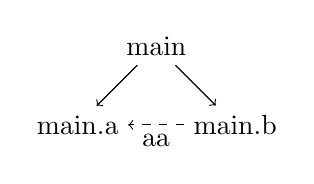
\begin{tikzpicture}
    \node[rectangle] (m) at (0,1) {main};
    \node[rectangle] (a) at (-1,0) {main.a};
    \node[rectangle] (b) at (1,0) {main.b};
    \path[->] (m) edge (a);
    \path[->] (m) edge (b);
    \path[->,dashed] (b) edge node[auto]{aa} (a);
\end{tikzpicture}

Another mechanism for managing name spaces is \emph{template 
inheritance}.  Using inheritance, one can create generic templates 
that capture common properties of a family of entities, leaving 
some of the properties underspecified.  The generic template can 
be specialised by a child template that fills in the missing 
details.  For example, the following template models common 
device-class callbacks that must be implemented by any OS 
specification for the IDE device class.  Note that callbacks are 
defined without bodies, as the exact behaviour is OS-specific.
\begin{tsllisting}{}
template ide_os
  procedure void write_sectors(uint<48> lba, 
    uint<16> sectors, uint<32> buf, bool xfer_error);
  procedure void read_sectors(uint<48> lba, 
    uint<16> sectors, uint<32> buf, bool xfer_error);
  procedure void reset();
  ...
endtemplate
\end{tsllisting}
This template is specialised by the \src{l4\_ide\_os} template,
that describes the IDE driver interface defined by the seL4 OS.
\begin{tsllisting}{}
template l4_ide_os(l4_ide_drv drv)
  // the derive statement is used to establish the 
  // inheritance relation
  derive ide_os;

  // additional specification items can be declared in the 
  // child template
  export iostatus reset_status = ionone;

  // the child template implements methods inherited from 
  // the parent.
  procedure void write_sectors(uint<48> lba, 
    uint<16> sectors, uint<32> buf, bool xfer_error)
  {
    assert (lba == r_lba);
    ...
  }
\end{tsllisting}



\chapter{Syntax reference}


\section{Import statements}

Import statements are used to combine multiple \tsl files into a 
single specification.  They are only allowed in the top-level 
syntactic scope, i.e., they are illegal inside template of type 
declarations.  An import statement consists of the \src{import} 
keyword followed by file path in angle brackets:
\begin{tsllisting}{}
import<ide_dev.tsl>
import<os/ide_tsl2/l4_ide.tsl>
import<../../os/ide_tsl2/ide_class.tsl>
\end{tsllisting}
The \tsl compiler appends this path to each import directory, 
specified via the \src{-I} command line switch, in order, until a  
file with this name is found.


\section{Templates}

Templates must be declared within the top-level scope, i.e., 
nested template declarations are not allowed.  Template 
declaration has the following syntax:
\begin{tsllisting}{}
template <template-name>[(<port-declarations>)]
  <template-item>*
endtemplate
\end{tsllisting}



\end{document}
